\documentclass[a4paper,twocolumn]{article}
\usepackage{natbib}
\usepackage{graphicx}
%\usepackage{pslatex}
\usepackage[margin=2.25cm]{geometry}
\usepackage{multirow}
\bibliographystyle{abbrvnat}

% opening
%% \author{Keegan Carruthers-Smith \\ \small{ksmith@cs.uct.ac.za}
%%         \and Julian Kenwood \\ \small{jkenwood@cs.uct.ac.za}
%%         \and Min-Young Wu \\ \small{mwu@cs.uct.ac.za}}

\begin{document}

\begin{titlepage}
\begin{center}

\includegraphics[width=100mm]{uct}\\
\ \\
\textsc{\Large
Department of Computer Science\\
\ \\
Honours Project Proposal\\
\ \\}
%
% the title
%
{\huge \bfseries
Improved Data Compression of Molecular Dynamics of Water
\\}
\ \\
\ \\

\begin{center}
  \begin{tabular}{lll}
    \large Keegan Carruthers-Smith & \large Julian Kenwood & \large Min-Young Wu
    \\
    \small{ksmith@cs.uct.ac.za} & \small{jkenwood@cs.uct.ac.za} & \small{mwu@cs.uct.ac.za} \\
  \end{tabular}
\end{center}

\vfill % fill vertical space
%
% Bottom of the page
% \today is the compilation date
{\large \today}
%
\end{center}
\end{titlepage}

\section{Project Description}
%{{{

There is no current system of compressing molecular dynamics simulations that
takes advantage of the special features of water. The current, more general,
compression scheme is also not considered to be very effective.

This project's goal is to develop a system that will take advantage of the
properties of water molecules in simulations. This system will be broken up
into three sections: \textit{Visualisation}, \textit{Connectivity} and
\textit{Compression}.


\subsection{Visualisation}
Quantisation compresses a range of values to a single quantum value, this makes
the data more compressible but the resulting data fidelity will be lower.

% how many points are we working with?

Being able to effectively visualise and analyse a millions of points in 3D
space is quite difficult. Techniques will need to be developed to allow the
user to see and analyse what is happening with the points in an easy to use
and intuitive manner.


\subsection{Connectivity}

\begin{figure}[!h]
\centering
\resizebox{0.45\textwidth}{!}{
  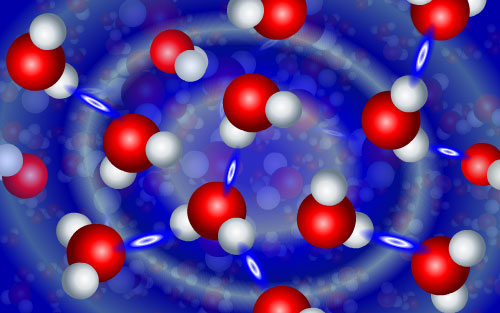
\includegraphics{watermol_flash.jpg}
}
\caption{Bonds between water molecules.}
\label{fig:water}
\end{figure}

The data given does not specify the bonds between the hydrogen and oxygen
atoms, but rather just the positions of each atom. A first step will be to
find these bonds. Now the problem is reduced to compressing molecules.

There are good heuristics on how water molecules are positioned relative to
one another. \ref{fig:water} shows an example bonding of water molecules.
Using these heuristics, a technique using \emph{predictors} can
be used to compress the point clouds. The predictors require a structure which
allow it to know what molecules to use to predict a new one. This is done by
creating a graph of the points, where the vertices are the molecules and the
edges indicate molecules than can predict each others position.

A spatial divisioning data structure will be used for more accurate creation
of the graph in the connectivity section. Some parts of space in the
simulation do not allow water to exist them, for instance inside other
molecules. These will be tested to see how worthwhile the trade-off between
the accuracy of the graph and the time and space efficiency is.


\subsection{Compression}


The core of the project is the compression of the molecular simulation
data. This will occur in several parts. The first is the creation and encoding
of the spanning tree from the original graph. The predictors used and the
given errors are encoded in order to faithfully recreate the spanning tree
when decompressed. The vertices of the spanning tree will represent the
molecules in a single frame of the simulation.

As well as single-frame compression, there will be multi-frame compression
techniques for subsequent frames in the simulation. Interframe predictors and
their residual errors will be encoded to achieve a better compression
rate. The frames that are predicted from previous frames will be grouped in
order to allow for random access into the simulation frames.


%}}}

\section{Project Statement}
%{{{

\subsection{What is being investigated?}

\subsubsection*{Visualisation}
\begin{itemize}
\item What is an acceptable level of quantisation?
\item How to effectively visualise and cope with large levels of detail?
\end{itemize}

\subsubsection*{Connectivity}
\begin{itemize}
\item Assuming what we know about water, can we exploit it to get good
  compression ratios?
\item Can we improve on the method employed by \citep{devillers2000gci}?
\item Can we improve on a na\"ive graph using heuristics?
\end{itemize}

\subsubsection*{Compression}
\begin{itemize}
\item What is the space and time efficiencies that are achievable in the
  compression of molecular dynamics simulations?
\item Is it possible to achieve better compression rates than other methods?
\item Is the amount of work required to construct the spatial divisioning data
  structure reasonable in the context of the performance of the compression
  algorithm?
\end{itemize}

\subsection{Why is the problem important?}

Molecular dynamics (MD) simulations generate vast amounts of data. A typical
100-million atom MD simulation produces approximately 5 gigabytes of data per
frame consisting of atom types, coordinates and velocities. This will generate
17 terabytes of data a day if run for 35\,000 steps with every 10th frame
being saved \citep{omeltchenko2000sls}. Generating this much data makes good
compression very desirable.

According to John E. Stone (Senior Research Programmer at Beckman Institute
for Advanced Science and Technology, University of Illinois) storing and
transferring the data produced by MD simulations is a major
hindrance. Efficient compression will help to alleviate the problem.

The level of quantisation plays an important part in determining the level of
compression that can be achieved. A higher resolution quantisation (large
number of bits used per point), will have higher data fidelity but will
correspondingly make compression harder and thus yield lower compression
rates. A lower resolution will yield a higher compression rate since there
will be less data to compress, but the resulting data fidelity may be too
low. Thus, a balance must be determined.

Being able to visualise the data is very important as the data being compressed
is very visual in nature (molecular simulation) and thus will not be easy to
understand in a non-visual manner (only seeing the point co-ordinates).


%}}}

\section{Related Work}
%{{{

\subsection{Visualisation}

Work has been completed on molecular visualisation, however the techniques
used are very specific to certain types of molecules; e.g. ribbon models for
proteins \citep{carson87} and twister for carbohydrates
\citep{kuttel06}. General visualisation techniques often have a different
problem domain and hence are not directly applicable, however the developed
techniques can be adapted. Examples would be clutter control \citep{ellis07}
and dealing with different levels of detail see Figure \ref{fig:clutter}.

\begin{figure}
\centering
\resizebox{0.45\textwidth}{!}{
  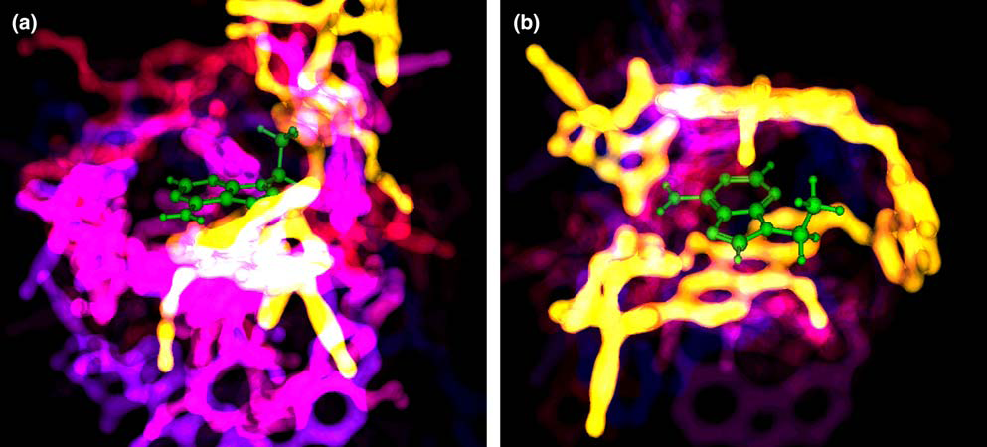
\includegraphics{cpictar.png}
}
\caption{An example clutter reduction scheme for molecule visualisation.}
\label{fig:clutter}
\end{figure}

% \centering
% \resizebox{0.9\textwidth}{!}{
%   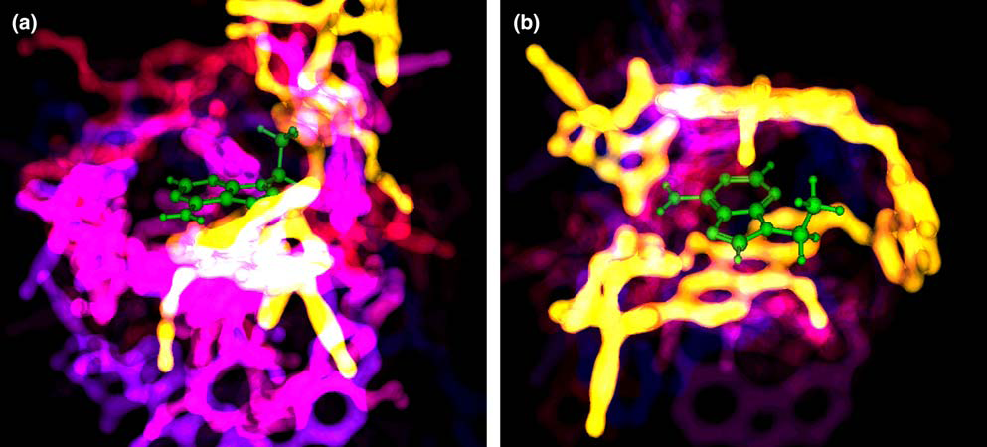
\includegraphics{cpictar.png}
% }

\subsection{Connectivity}

\begin{figure}[!h]
\centering
\resizebox{0.45\textwidth}{!}{
  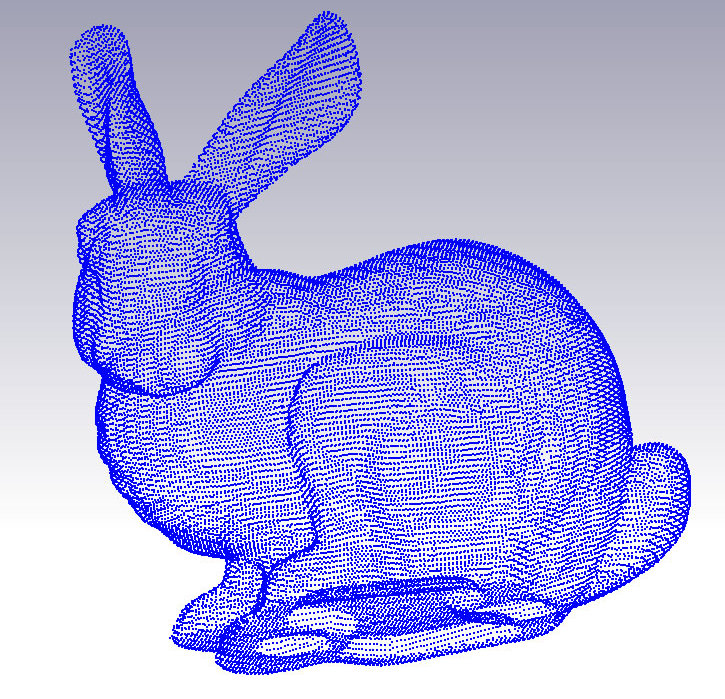
\includegraphics{bunny.jpg}
}
\caption{An example clutter reduction scheme for molecule visualisation.}
\label{fig:points}
\end{figure}

Most research on point clouds involves point clouds of surfaces. 
Figure \ref{fig:points} shows a point cloud of the surface of a rabbit. This is
because most point clouds are obtained from 3D scans of object surfaces. A
surface is the “skin” of an object, i.e. the boundaries of a solid
object.

Since point clouds don not have any connectivity information, connectivity has
to be added in a heuristic manner. The heuristics developed in the field
exploit the nature of the surface scans of objects.

\cite{gumholdcomp} create a tree of the points that exploits the knowledge
that the points lie on a surface. They do not, however, use predictors which
exploit this. \cite{merrycomp} extend on this by using predictors which do
exploit the rectilinear nature of surface scans.

\subsection{Compression}

There has been previous work by \citep{omeltchenko2000sls} that has been
performed into compressing molecular simulations. This research used several
techniques to provide better compression rates. The space the simulation
exists in is quantised into a grid of cells. Atoms are snapped to the center
of their nearest grid cell. These cells are then indexed using a space-filling
curve called octree indexing. The atoms are sorted in increasing order of
their cell index. These indices are then differentially encoded using a
variable-length encoding scheme. There is, however, no attempt to make use of
the characteristics of water in this approach.


%}}}

\section{Procedures and Methods}
%{{{

\subsection{Implementation Strategy}

\subsubsection*{Visualisation}

The first step in visualisation will be determining the acceptable level of
quantisation. This will involve the users of the system to determine what the
`acceptable' level is. The result from this will be used in the compression
part of the project. Whether this data is available or not will have minimal
effect on the actual compression process.

The next step in visualisation will depend on the completion of the
compression and decompression aspect of the project; however, as the interface
between the visualisation and decompression will be well defined, the
visualisation can be tested with auto generated data.

A prototype will be developed for the initial testing of the visualisation
technique and clutter control, this will allow for the idea to be quickly
tested, refined and evaluated.

\subsubsection*{Connectivity}

This first step will receive a quantised point cloud of hydrogen and oxygen
atoms. This will be transformed into a point cloud of water molecules. This is
known as \emph{bond extraction}.

Then a graph over the molecule points will be created. This graph will have
edges between points that are close to one another. The na\"ive algorithm will
just use the Euclidean distance to determine ``closeness''. The final
algorithm will use a different metric to determine ``closeness''. It will take
into account the predictors we have about how water molecules bond. If a
predictors predicts another molecule well, it is ``closer'' than a molecule
which is predicted less effectively.

This graph will also use heuristics to reduce the number of edges in the
graph. This is for improving the space and time efficiency of the
algorithm. From what is known about water, there is an upper bound on the
``closeness''. Limiting edge length to be less than the upper bound, the graph
becomes a multi-graph of connected components. We plan on na\"ively connecting
the components. A possible extension would be to encode the components
separately, and see how that improves compression.


\subsubsection*{Compression}

% Discuss Arithmetic Coding, Spanning Tree Encoding, Spatial Decomposition Data Structures

The compression side of the project will utilise Arithmetic Coding as the
compression backend. Arithmetic Coding is an optimal variable-length encoding
scheme that can be used to compress arbitary data. The mechanism that is used
to accomplish this is complicated and we may use software package to perform
the actual compression for prototypes or, possibly, the finished project.

In the connectivity part of the project a graph structure for the
underlying water molecules is created. This graph structure will then
be encoded using a spanning tree approach. A spanning tree for the graph will
be constructed and various predictors will be used in order to provide better
compression rates.

The graph that is created to represent the water is not exact. The non-water
molecules may not contain any water molecules. A spatial divisioning data
structure, such as an octree, can be used to better help construct the graph
more accurately by eliminating the area of space that the water molecules may
not exist in. By eliminating these possibilities from the graph it may be
possible to achieve better compression rates. The construction time of the
data structure may be too large to justify any increase in compression rates
so we will be examining the benefit of the data structures.

The initial prototype of the compression component will only include the
Spanning Tree encoding and use a plugin arithmetic coder component. The
spatial divisioning data structure will initially consist of stubs that will
return a 'no collision' result for all tests. These features will be built-up
in further prototypes.

% Unit testing will be performed on all of these components. The spanning tree
% encoding will tested with various graphs. The tests will ensure that the
% graph can be reconstructed properly. The spatial divisioning data structure
% will consist of

In order to evaluate whether the compression scheme is successful or not,
various statistics will be gathered. The compression ratio of the system will
be measured as well as the time and space requirements. Finally, a comparison
between the two systems with and without the spatial-divisioning data
structure will be conducted in order to determine which one is better.


% a) Prototype features
% b) Testing plan
% c) No mathematics for me

\subsection{Testing}

\paragraph{Visualisation}
To determine an acceptable level of quantisation, user evaluation and
communication will be conducted. The results from the different levels of
quantisation will be presented and a knowledgeable user will be asked to
comment on the results.

The visualisation will be tested with user evaluation. Users will be asked to
use and comment on the visualisation technique used to present the data.

\paragraph{Connectivity}
A simple script will be created to generate random test data. The data will be
already quantised (and different levels of quantisation can be applied). Then
a script will be created to test the output graph. The graph must satisfy the
following
\begin{itemize}
\item A one to one correspondence (w.r.t location) between molecule vertices
 and atoms in the generated point cloud.
\item The graph must be connected.
\end{itemize}

The tests will also be carried out on sample data from MD simulations.

\paragraph{Compression}

Several metrics will be used to test the success of the software compression techniques. Performance measurements will be used to determine the space and time efficiency of the compression scheme. A determination of the time taken to encode a single frame of a molecular simulation as well as the time to compress all frames. These measurements will give insight into the amount of resources required for a reasonable compression rate.

The compression rate will also be checked for each of these performance measurements. It will then be possible to measure the effectiveness of the compression scheme with respect to previous works.

The success of the spatial divisioning data structure will be tested by
comparing the compression rates and time and space efficiency. The rates that are 
achieved with and without the data structure will be measured. A significant increase
in compression rate with moderate increase in space and time will indicate a
successful trade-off.

%}}}

\section{Ethical, Professional and Legal Issues}
%{{{

This is for the benefit of the scientific community, so will be made available
in the public domain. The product is also likely to be included in some form
in VMD.\citep{VMD} So the product will eventually be part of the Open Source
community.


\paragraph{Visualisation} For the visualisation side of things, there is the
concern that people may become nauseous from using the visualisation; however
this is not likely in the case of this project as the user will not be
interacting with the visualisation, they will only be watching the
visualisation.

\paragraph{Connectivity} There are no issues related to this.

\paragraph{Compression} There exists several patent issues that exist with
Arithmetic Coding compression schemes, however, these patents have mostly all
expired.

%}}}

\section{Anticipated Outcomes}
%{{{

\subsection{System}
\begin{itemize}
\item A standalone visualisation program will be developed which will be used
  to view the compressed data.
\item A compression and decompression program for MD data formats.
\end{itemize}

\subsection{Expected impact}
It is expected that we shall improve on existing methods for point cloud
compression and molecular dynamics compression.

\subsection{Key success factors}

\subsubsection*{Visualisation}
\begin{itemize}
\item Acceptable levels of quantisation will be determined.
\item The visualisation technique employed will be acceptable, as determined from user testing.
\end{itemize}

\subsubsection*{Connectivity}
\begin{itemize}
\item Do we achieve better compression ratios than other methods?
\item Do we compress in an efficient manner? We aim for the compression
  algorithm to be in $O(P^2)$ where $P$ is the number of points.
\item Do we decompress in an efficient manner? We aim for a decompression
  algorithm in $O(P)$.
\end{itemize}

\subsubsection*{Compression}
\begin{itemize}
 \item Do we achieve good space and time efficiency with reasonable compression rates? 
 \item Do we perform better than other methods? The previous simulation encoding scheme acheived a compression rate of approximately 6 bits per atom. \citep{omeltchenko2000sls}
 \item Does the spatial divisioning data structure provide a good trade-off? 
\end{itemize}



%}}}

\section{Project Plan}
%{{{

\subsection{Risks}
\label{sec:risksection}

Refer to table \ref{tab:riskfactors}.

\begin{table*}[h]
  \begin{tabular}{|p{7cm}|c|c|c|}
    \hline
    \textbf{Factor} & \textbf{Probability} & \textbf{Impact} & \textbf{Risk} \\
    \hline
    
    Not receiving MD simulation data & Low & Medium & Low \\ \hline

    Losing source code & Low & Medium & Low \\ \hline
    
    Project requirements changing & Low & High & Medium \\ \hline
    
    Project member dropping out & Low & Medium & Medium \\ \hline

    Running behind schedule & Medium & Medium & Medium \\ \hline

  \end{tabular}
  \caption{Risk Factors}
  \label{tab:riskfactors}
\end{table*}

\subsubsection*{Mitigation}

We plan on using an iterative development methodology. This is to identify
unknown risks early on so we may deal with them. The following are how we will
deal with the risks we have already identified.

\paragraph{Not receiving MD simulation data.} We can create our own random
data sets based on our heuristics. This will give high compression ratios,
which makes our compression ratios results void. But it can still test
efficiency and quantisation.

\paragraph{Losing source code.} We will be using Mercurial for source
control. This is a distributed system, so copies of our code will be stored on
multiple machines. These machines will also be geographically separated. So we
can restore from another machine if the code is lost.

\paragraph{Project requirements changing.} We will be having regular meetings
with our supervisors. This will ensure we are up-to-date with any changes that will affect our project requirements.

\paragraph{Keegan dropping out.} Julian can apply only inter-frame
compression, without the predictor compression. Most of the work load could
also be split between the remaining members, and the goals reduced.

\paragraph{Julian dropping out.} Keegan can implement the predictors. We can
then do no inter-frame compression, just do the predictor compression every
frame. Min-Young can implement the reference compression method by
\citep{omeltchenko2000sls}.

\paragraph{Min-Young dropping out.} Keegan or Julian can implement a simple
quantisation. No experiments will be done regarding varying levels of
quantisation or on visualisation.

\paragraph{Running behind schedule.} We have three milestones, to reduce the risk
of falling behind schedule. We may also simplify the compression and
visualisation approach if we fall vastly behind schedule.

\subsection{Timeline}

For the timeline see Figure \ref{fig:timeline}, for the tasks see Figure \ref{fig:tasks}.

\subsection{Resources required}

\subsubsection{People}

\paragraph{Dr. Patrick Marais} Patrick is a co-supervisor that will be involved
with general guidance for the project.

\paragraph{Dr. James Gain} James is a co-supervisor that will be be involved
with general guidance for the project.

\paragraph{Dr. Michelle Kuttel} Michelle will be providing guidance on the
heuristics that will be used in the compression algorithm. She can also provide sample molecular simulations to test our program with.

\subsubsection{Software}
Molecular simulation data will be needed to test the project with, this will.
Without the test data, the project will be able to
continue but the results may not be applicable anymore. This risk has been
assessed in the Risks section. (Section \ref{sec:risksection}).

C++ will be the language used for the implementation. The following libraries
will be used by the program:
\begin{itemize}
 \item An arithmetic encoding library, such as \citep{AC} - for the compression backend 
 \item OpenGL - for rendering the visualisation
\end{itemize}

% are we using any libraries?

\subsubsection{Equipment}
% what are we!? Developers? Implementors? Authors? Researchers?

Development will be completed on the personal computers of the developers and
the desktops provided by the university. GNU/Linux will be the system used for
development, as well as the target system.


\subsection{Deliverables}

The deliverables for the project will contain software to compress, decompress
and visualise the molecular data. Three individual reports will also be
produced to accompany the softare, detailing the three different sections of
the software. A single poster and website will also be produced. Finally, there
will be a presentation to demonstrate the project as a whole.


\subsection{Milestones}

See Table \ref{tab:milestones} for the milestones.

\begin{table}
  \centering

  \begin{tabular}{|c|c|p{4cm}|}
    \hline
    \textbf{Section} & \textbf{Date} & \textbf{Milestone} \\
    \hline \hline
    \multirow{4}{*}{Coding} & 30-31/7 & Feasibility Demonstration \\
 & 2/10 & First Prototype Implementation Finished \\
 & 16/10 & Final Prototype Implementation Finished \\
 & 23/10 & Coding Complete \\
 \hline
 \multirow{13}{*}{Report} & 8/5 & Literature Survey \\
 & 18/5 & Project Proposal \\
 & 18/5 & Project Plan\\
 & 22/5 & Proposal Presentation \\
 & 25/5 & Finalised Proposal \\
 & 31/7 & Background/Theory Chapter \\
 & 4/9 & Design Chapter \\
 & 2/10 & First Prototype Writeup Finished \\
 & 16/10 & Final Prototype Writeup Finished \\
 & 23/10 & Implementation and Testing Chapter \\
 & 27/10 & Complete Report Outline \\
 & 30/10 & First Report Draft \\
 & 6/11 & Project Report \\
 \hline
 \multirow{5}{*}{Other} & 13/11 & Web Page \\
 & 13/11 & Reflection Paper \\
 & 13/11 & Poster \\
 & 16-18/11 & Demonstration \\
 & 23-24/11 & Final Presentation \\
 \hline

\end{tabular}
\caption{Milestones for the project}
\label{tab:milestones}

\end{table}


\subsection{Work allocation}

\paragraph{Min-Young Wu} \emph{Visualisation} - Visualisation Program,
Quantisation and Quantisation Experimentation.
\paragraph{Keegan Carruthers-Smith} \emph{Connectivity} - Bond Extraction and Graph
Creation.
\paragraph{Julian Kenwood} \emph{Compression} - Spanning Tree Creation,
Predictors, Spatial Divisioning Data Structures, Multi-Frame Compression and Decompression

%}}}

\bibliography{proposal}

\begin{figure*}[!h]
\centering
\resizebox{0.7\textwidth}{!}{
  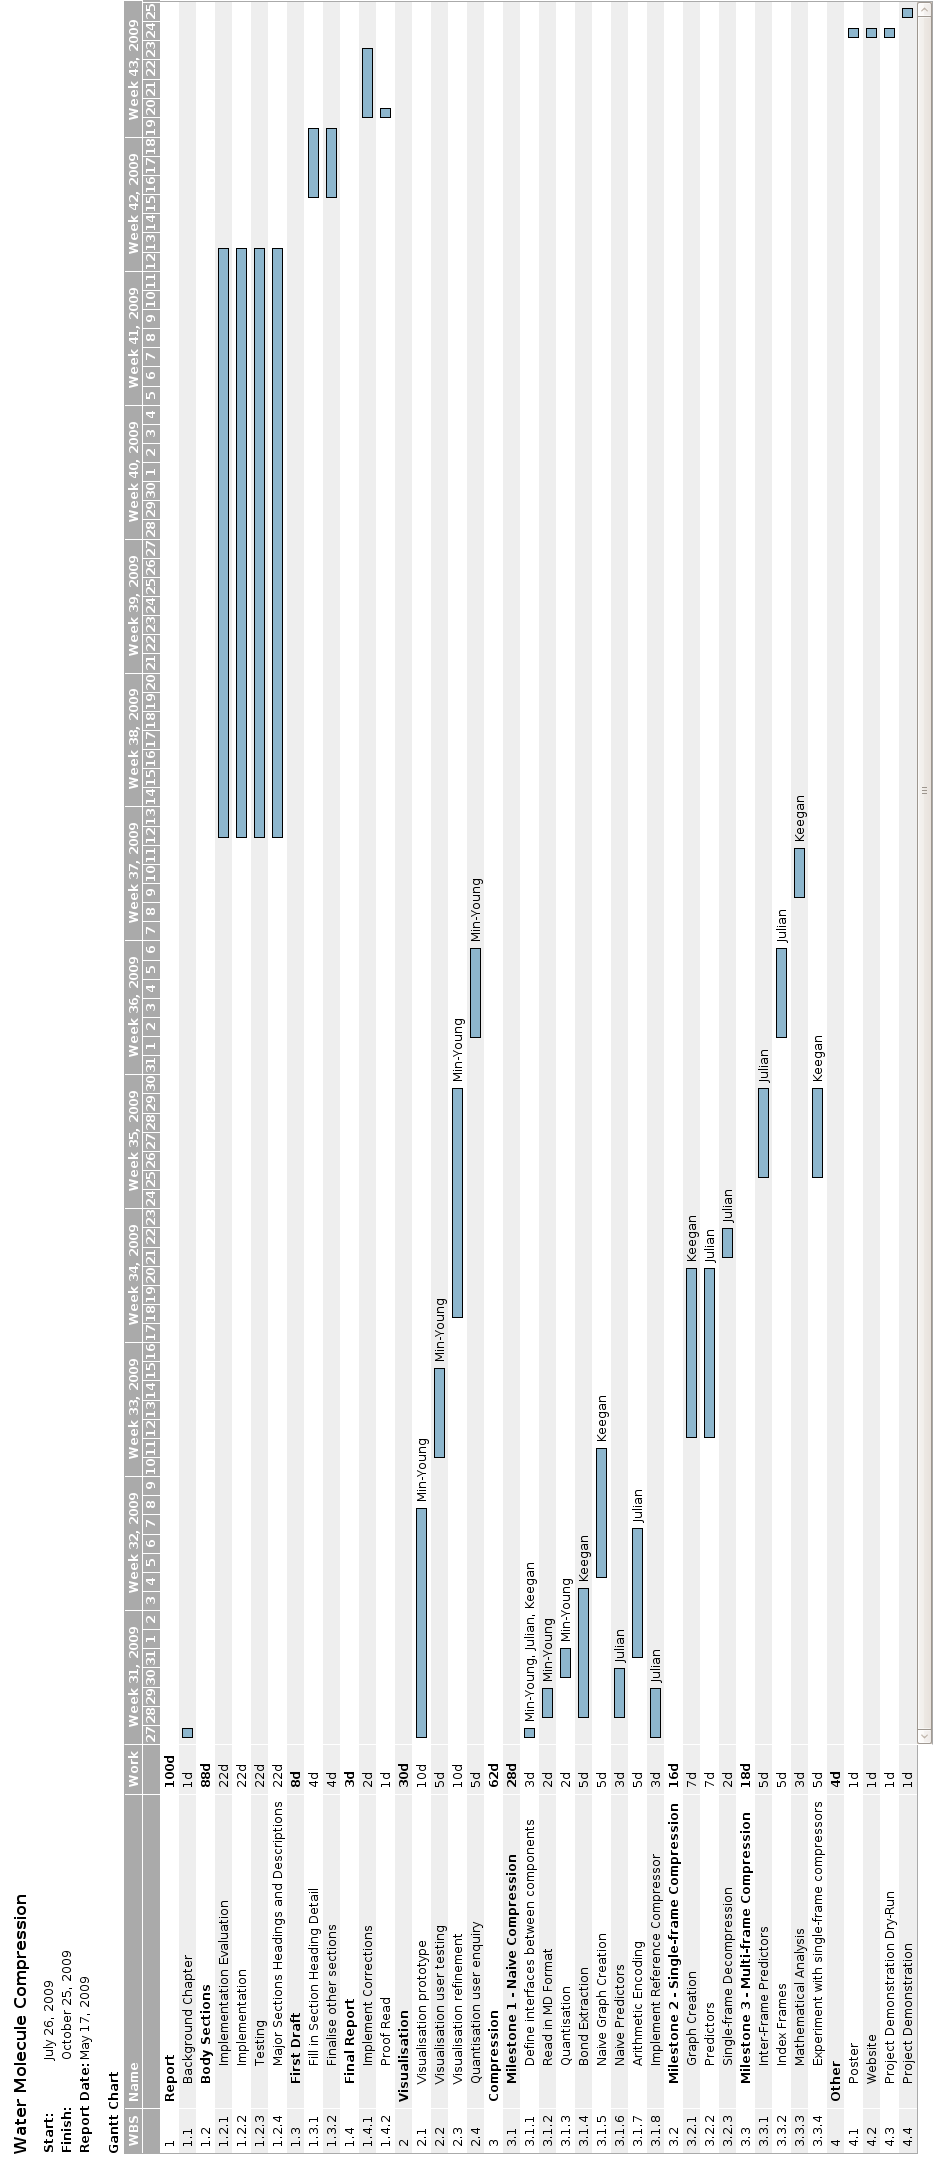
\includegraphics{chart.png}
}
\caption{Timeline of the project.}
\label{fig:timeline}
\end{figure*}

\begin{figure*}[!h]
\centering
\resizebox{0.95\textwidth}{!}{
  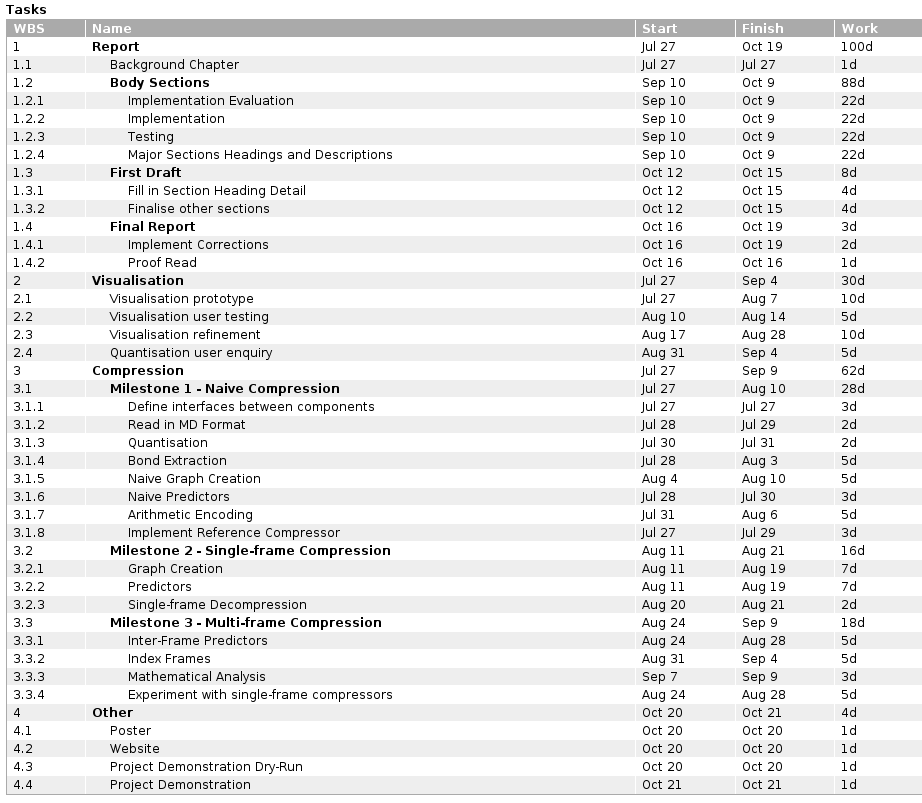
\includegraphics{tasks.png}
}
\caption{Tasks for the project.}
\label{fig:tasks}
\end{figure*}

%\nocite{*}

%\bibliographystyle{acm}

\end{document}
